% Copyright (c) 2014,2016 Casper Ti. Vector
% Public domain.

\chapter{引言}

\section{分布式图处理系统}
互联网的飞速发展产生了海量的数据,特别是最近几年智能移动设备的快速普及,更使得数据呈爆炸式增长。在大数据时代,海量数据的处理需求已远超单台机器所能提供的性能,为此人们在廉价的商用机集群上构筑了各式各样的分布式系统,以获得可靠、可扩展的海量数据处理能力。在各种数据表示方式中,图(Graph)由于其丰富的表达能力而得到了广泛应用。图中的顶点可以表示实体,图中的边表示实体间的关系。社交网络、语义网络、生物信息网络是典型的图应用场景。
图数据分析与处理是大数据背景下的一大研究分支\supercite{big_data},大数据背景下的图处理系统可以分为图计算框架和图数据库两大类。

图计算框架旨在高效地进行全图量级的并行计算,如计算PageRank\supercite{pagerank}、社区发现\supercite{community_detection}(Community Detection)、子图匹配\supercite{subgraph_listing}等,提供对全量数据进行离线计算的解决方案。这类系统中,Pregel\supercite{pregel}、Giraph\footnote{Giraph, https://giraph.apache.org/}支持BSP\supercite{BSP}(Bulk Synchronous Parallel)模型的计算,将图计算表示为以点为中心的计算模型,各节点在完成自己的计算后,在每个Super Step中同步自己的计算结果到邻居结点中。BSP模型的缺点在于每个Super Step需要严格同步,如果有节点处理速度较慢,将直接拖慢整个系统的处理速度。另外每个节点的更新在一个Super Step内只能传播到邻居节点,需要多个Super Step才能将更新的影响传播到全图中。GraphLab\supercite{graphlab}是另一个高性能的图计算框架,其抛弃了BSP模型,使用异步动态更新(Asynchronously Dynamic Update)来传播计算节点间的结果。区别于Pregel和Giraph使用边分割来划分子图,GraphLab使用点分割来划分图数据,每个计算节点处理一个子图,各计算节点间的子图是有边界点作为交集的。各计算结点只需要交换边界节点的计算更新,子图内的更新可以异步地在本地传播。GraphLab精妙地控制节点间的异步更新以保证算法的收敛。PowerGraph\supercite{powergraph}是在GraphLab的基础上进行改进的图计算框架,其更适合处理自然界中普遍存在的满足Power Law的图数据。GraphLab和PowerGraph把图计算框架的性能提高到一个新的高度,但其容错性的处理欠佳,而且无法有机地融入已有的大数据生态系统中,往往需要单独部署和单独维护。GraphX\supercite{graphx}解决了这个问题,其是基于分布式内存计算框架Spark\supercite{spark}实现的图计算引擎,设计思路借鉴了GraphLab和PowerGraph。GraphX使得图计算可以融入整个数据流处理的框架,在Spark上提供了一栈式的解决方案。相对于分布式计算框架,GraphChi\supercite{graphchi}则追求在单机完成大规模图数据的计算问题。GraphChi只支持异步模型,从而能够合理组织更新来避免磁盘的随机IO请求,通过磁盘的顺序操作使磁盘达到接近内存的性能,从而能在单机上实现大图数据的计算。在图计算领域还有许多研究旨在提高图计算框架在特定问题的处理性能,如\supercites{xuning_LogGP,xuning_2,shaoxia_1,shaoxia_2,shaoxia_3}等。学术界对图计算的研究热情普遍高涨。

图数据库专注于图数据的管理,提供高效的图遍历查询(graph traversal)。图数据模型则是指图数据库如何以图的方式对数据进行抽象 \supercite{graph_models_survey},应用较广泛的图数据模型有RDF\footnote{RDF 1.1 Concepts and Abstract Syntax, https://www.w3.org/TR/rdf11-concepts }模型和属性图\supercite{property_graph}模型。RDF全称为Resource Description Framework,是由W3C制定的知识描述标准,使得按RDF表示的不同数据源可以进行数据交换或合并。RDF中的数据单元是由主语、谓语、宾语组成的三元组,可以直接对应为图上的一条边,因此将RDF模型归类为图数据模型。
著名的RDF数据库有Yago\supercite{yago}、DBpedia\supercite{dbpedia}、ProBase\supercite{probase}等。
当今的图数据库大都采用属性图模型设计\supercite{graph_database_models},如DEX\supercite{DEX}、GraphChi-DB\supercite{graphchi-db}、Neo4j\supercite{neo4j}、Titan\footnote{Titan, http://titan.thinkaurelius.com}等,其中DEX和GraphChi-DB都只是单机数据库,Neo4j的开源版本也是单机的,只适合处理中等规模的图。Titan则是目前应用广泛的分布式图数据库,由于其完全开源免费,因此在社区中得到了广泛关注,也是本文的研究对象。Titan的底层实现了可插拔的存储接口,可部署在HBase\footnote{Apache HBase, http://hbase.apache.org }、Cassandra\supercite{cassandra}或BerkeleyDB\footnote{Oracle Berkeley DB Java Edition, http://www.oracle.com/technetwork/database/berkeleydb }之上,因此可以很好地与Hadoop\footnote{Hadoop, http://hadoop.apache.org }集群结合,融入已有的大数据生态系统,组成统一的数据处理框架。
%然而,现有的图数据库都没有考虑含有大量重边的属性图应用场景。HybriG架构填补了这个空白,为含有大量重边的属性图应用场景提供了一种可行的解决方案。

\section{传统图数据库及其局限性}
传统图数据库大都以属性图作为数据模型。在有向图中,如果两条边具有相同的起点和终点,则称这样的边为重边(multi-edge)。属性图\supercite{property_graph}是一种带重边的有向图,图中的每个元素(点/边)可以拥有任意数量的属性值。特别地,每个元素都有一个label属性,标识该元素的类别。

图数据可以存储在关系数据库中,如把图中的边(即各类关系)存储为实体关系表,实体的信息存储为实体数据表。关系型数据库能胜任图数据的存储,也能方便地检索元素的内容,但在图结构相关的查询上表现欠佳。图结构相关的查询是指与图中的邻接关系(即图的拓扑结构)相关的查询,如多跳邻域查询、路径查询、子图查询等。关系数据库常常需要把图结构相关的查询转换为关系表的JOIN操作。比如两跳邻域查询,给定一个实体,查看其两跳范围内的子图。由于关系表只存储了图中的边,即只存储了一跳的邻域信息,为得到第二跳的邻域结点,需要对关系表做昂贵的JOIN操作。如果图中含有多种类型的边,则关系数据库中将维护多张实体关系表,实际转化出来的JOIN操作将更为复杂。图数据库由于其以图的形式存储数据,因此能高效地检索各点、边的拓扑信息,在这类图结构相关查询中就具有更优异的性能。另外,图数据库也能高效地支持点、边属性的查询。因此当应用场景中图的拓扑结构查询与元素的内容查询同等重要时,图数据库是最佳的选择。

实际应用中,有些属性图会含有大量重边。比如在电信行业的通话关系图中,两人之间可以发生多次通话关系;又比如金融行业的交易关系图中,两人之间可以发生多次交易关系。更复杂的,在刑侦应用中,整个情报系统获得的信息融合成一个知识图谱\supercite{knowledge_graph},其中的实体和关系类型丰富多样。比如实体类别有人、汽车、公司等,实体间的关系有亲属关系、共同出行关系、通话关系等。有的关系是可以多次重复的,频次可能成百上千,这使得两个实体间不仅有多种label(即多种关系)的边,还包含大量重边。图\ref{fig:property_graph}是属性图在刑侦场景中的一个简单示例,显示了类型为人的结点以及通话关系和共同出行关系。其中共同出行关系是双向的,因此在图中以无向边表示。刑侦场景中的典型查询包括了元素信息查询和图结构相关查询,比如从一个人出发查询与其相关的所有人(邻域点集查询)、查询两个人在几跳内是否有关系(路径查询)、查询两人之间的所有关系(两点间边集查询)等。

\begin{figure}[htbp]
\centering
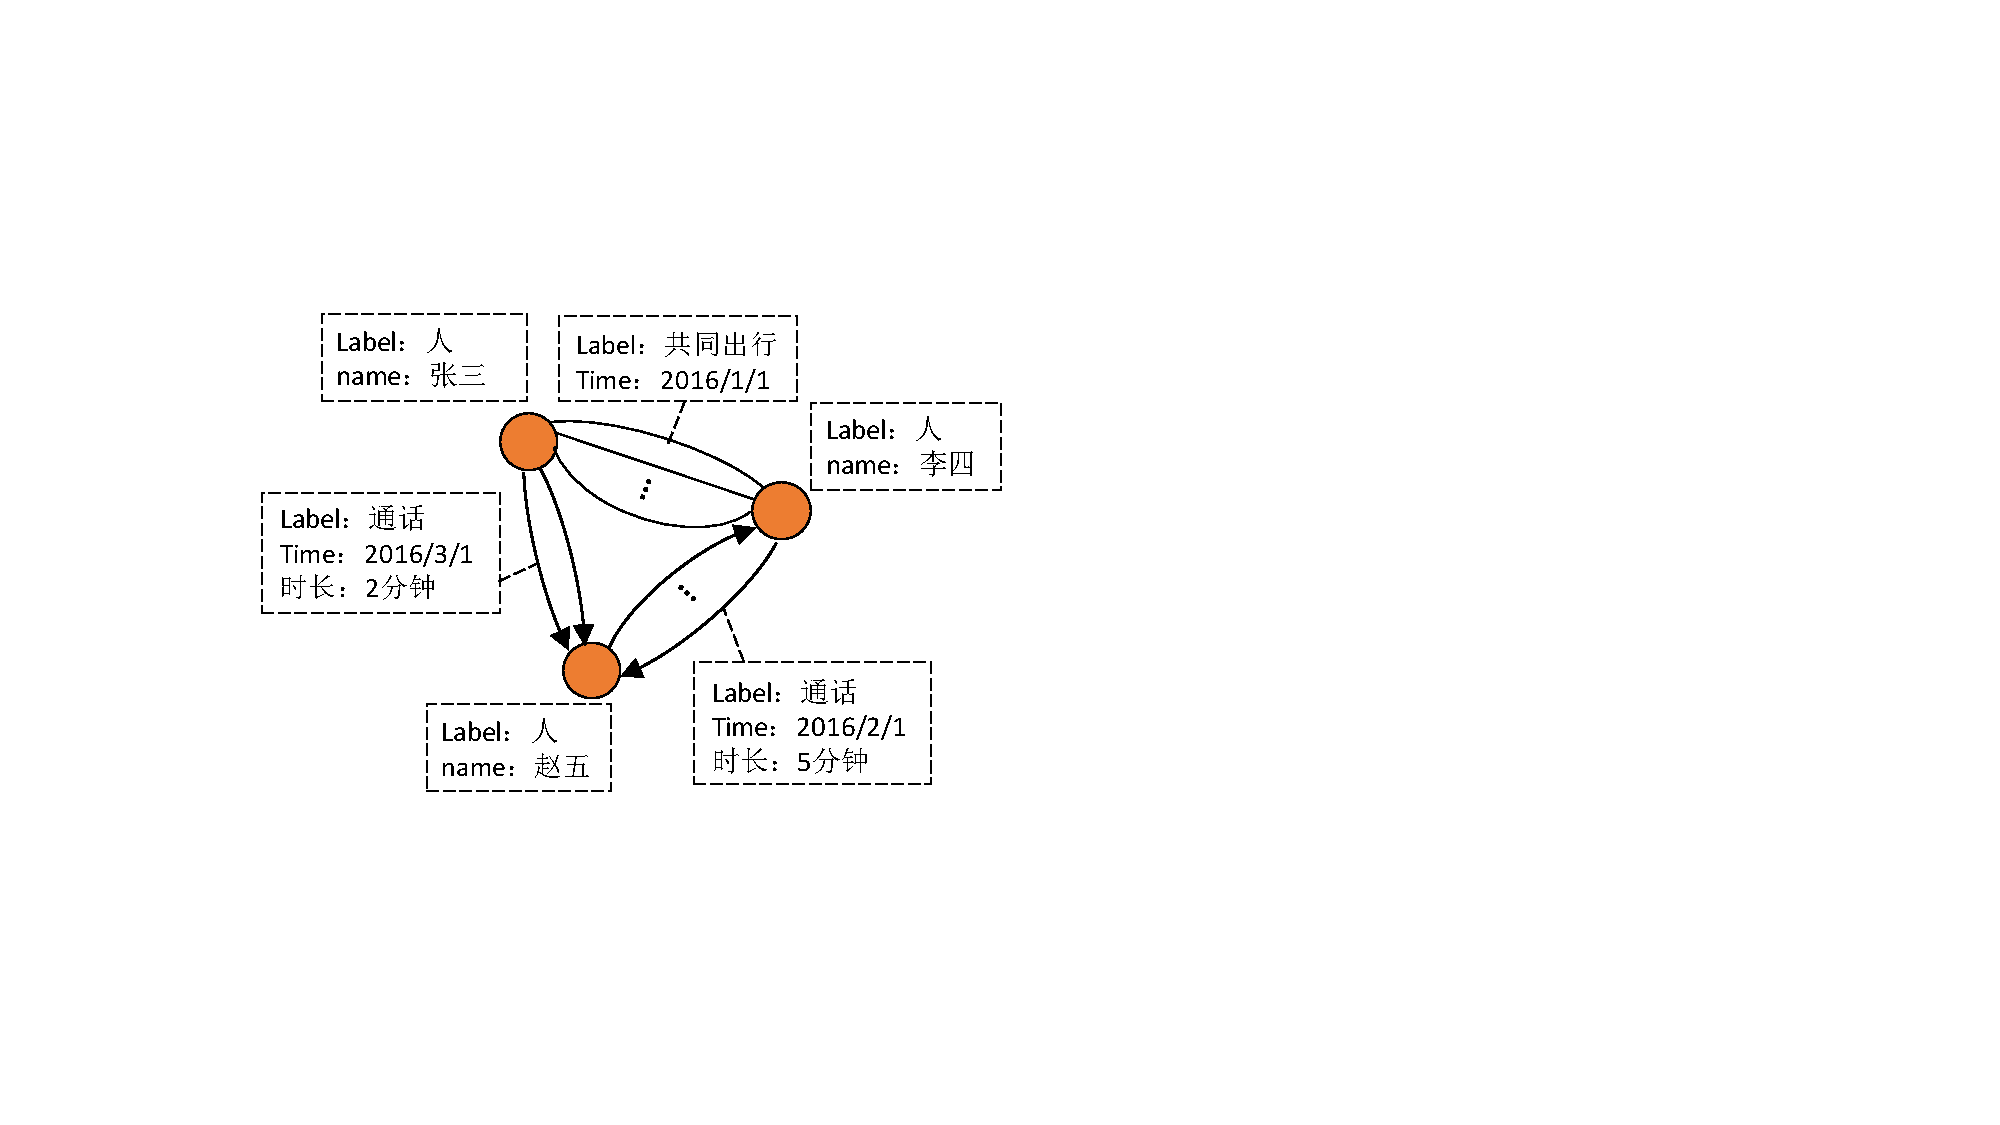
\includegraphics[width=100mm]{fig/property_graph.pdf}
\caption{属性图示例}
\label{fig:property_graph}
\end{figure}



然而,在富含重边的属性图中,图数据库的查询性能不佳。图数据库以邻接表的方式存储图,表中的每一项存储一条边。这使得查询邻接点集时,需要遍历整个邻接表中的所有边,而查询目标只是这些边里邻接的点集数据。当重边规模巨大时,这些邻接点大量重复,遍历这些邻边所带来的开销将不可忽略。邻域查询是大部分图查询的基础,如多跳邻域查询、路径查询、局部聚集系数查询(计算)等,这些查询往往由嵌套的邻域查询实现,随着邻域深度的增加,这些查询的性能将有指数级的降低。

为了避免在图数据库中处理大量重边,一种简化重边的建模方式是,将所有同label(即同类型)的重边合并为一条边来表示,合并后的边上存储这些重边的所有数据,这样两个实体间的重边数能降低为边的label种类数。然而,图数据库中将一条边作为一个存储单元,如果将多条重边的数据合并在一条边中存储,会使边的单位数据量骤增,图中的数据粒度过大。每次读写原图中一条边时,需要把合并的重边数据都读出来进行读写,降低了单条重边的检索和插入效率。因此,处理大量重边是一个不可避免的需求。而图数据库在处理该场景时有其局限性,因此本文提出了HybriG存储架构来优化传统图数据库在该场景的应用。

\section{HybriG存储查询架构}

HybriG是本文提出的一种复合存储架构,其基于Titan和HBase建立存储层,能克服传统图数据库的局限性,高效处理属性图中的大量重边。其中Titan是应用广泛的分存式图数据库,HBase是一个分布式的列式存储数据库。在HybriG架构中,我们将图中的重边数据存储于HBase里,图中的点集数据和点集间的连接信息则仍存储在图数据库Titan中。HybriG能从容地处理富含重边的属性图,当图中重边的规模巨大时仍能保持精简的邻接表,从而提供高效的邻域查询实现,进而能高效地支持更高级的图查询。虽然边集数据被拆开存储于HBase和Titan中,边集相关查询需要联合两个底层存储的查询结果,但HybriG通过合理的查询转化,使得边集查询的性能仍与传统Titan图数据库的性能相当。另外,HybriG架构的邻接表存储的是点集的相连信息,可以在其中预存重边的统计信息,从而能高效地支持重边上的一些统计查询。

HybriG架构相比于传统图数据库Titan,简化了对事务的支持,这主要是因为应用场景对事务没有很强的需求。在许多富含重边的图应用场景中,边集数据常常是事件类型的数据,即代表客观事实,无需修改。因此边集数据的操作需求相对单一,只有插入操作和后续的查询操作,没有很强的事务性要求。比如在知识图谱的构建中\supercite{knowledge_graph},信息的来源是可靠的,即一旦信息进入知识图谱,则被认为是无需修改的,因此数据操作只需要插入和查询,更新操作很少被执行。在刑侦应用场景中,数据来源是可靠的,且图中数据都是一些客观的事实数据,都由可信部门采集而来,不需要修改,数据操作主要是图查询和批量的图数据插入。数据插入操作包括原始的全量数据导入和定期的增量数据导入,没有并发的写冲突,也不需要很强的事务性要求。基于上述观察,HybriG放宽了对强事务的支持。
HybriG支持点集数据的事务操作,在边集插入上需要应用程序规避写-写冲突,但保证边集数据的最终一致性。这是因为HybriG将边集数据分开存储在Titan和HBase两个存储中,只保证二者数据的最终一致性。HybriG的事务支持足以满足大部分应用场景的需求。


本文的贡献主要有:

\begin{itemize}
  \item 分析了图数据库处理大量重边时查询性能受损的原因。其本质原因是图数据库邻接表中的存储单元是图中的一条边。无论邻接表中边集的排序如何设计,总能找到特定的邻域查询,使得其实现需要遍历整行邻接表。而基于邻域查询的高级查询将有指数级的性能下降。
  \item 基于上述观察提出了解决方案HybriG及其存储、查询和高效数据导入设计。解决了HybriG架构中异构存储的一致性问题,提出了保证最终一致性的数据导入设计。
  \item 通过实验验证了HybriG的优异性能。HybriG在邻域点集相关查询以及数据批量导入上相比传统图数据库Titan具有更优异的性能,在边集查询上与Titan性能相当。
\end{itemize}

\section{文章组织结构}
本文组织如下:第\ref{chap:related}章介绍图数据库相关的预备知识,包括HBase及Titan的实现及其在处理大量重边时的局限性;第\ref{chap:design}章介绍HybriG的系统架构,包括所支持的各种查询的设计与实现,数据高效导入方案的设计,以及数据一致性的设计;第\ref{chap:experiments}章展示相关的实验结果。

% vim:ts=4:sw=4
